\subsection{Anwendungsfälle modellieren}
\label{sec:Kap-6.3.1}

Bei der Modellierung von Anwendungsfällen (engl. use case) geht es darum, was Nutzer mit dem Softwareprodukt tun möchten bzw. tun. Anwendungsfälle werden daher verwendet, um ein Modell der Systemnutzung zu erstellen. \marginline{Modell der Systemnutzung} Dafür betrachten sie auf einer sehr hohen Abstraktionsebene die Interaktion verschiedener (potentieller) Nutzergruppen mit dem (zu erstellenden) Softwaresystem. Der Fokus liegt somit nur auf den extern sichtbaren Funktionalitäten des Systems und betrifft insofern eine Teilmenge der funktionalen Anforderungen. Über die Anwendungsfälle werden die Wünsche der Nutzer an die Software erfasst und dokumentiert. Das System selber wird als Blackbox behandelt, nur die Interaktion zwischen Nutzer und System wird betrachtet. Von den modellierten Anwendungsfällen ausgehend können dann im Entwurfsprozess der Software andere Arten von Diagrammen verwendet werden, um das dynamische Verhalten des Systems während der Interaktion mit dem Nutzer darzustellen. 

Das Anwendungsfalldiagramm der UML (engl.: use case diagram) basiert auf den Arbeiten von Ivar Jacobson in seiner Object-Oriented Software Engineering (OOSE)-Methode \cite{jac92}. Anwendungsfalldiagramme dienen in erster Linie der Kommunikation zwischen Nutzern und dem Softwareentwicklungsteam. Sie sind sehr einfach gehalten, damit sie auch von technisch nicht-versierten Nutzern verstanden und erstellt werden können. Abbildung~\ref{fig:fahrkartenautomat} zeigt ein erstes, noch sehr basales, UML-Anwendungsfalldiagramm.

%hier gehört abb Anwendungsfalldiagramm ("fig:fahrkartenautomat") eigentlich hin
\begin{figure}[h!]
	\vspace{\baselineskip} %%% für Druck
	\vspace{\baselineskip} %%% für Druck

	\centering
	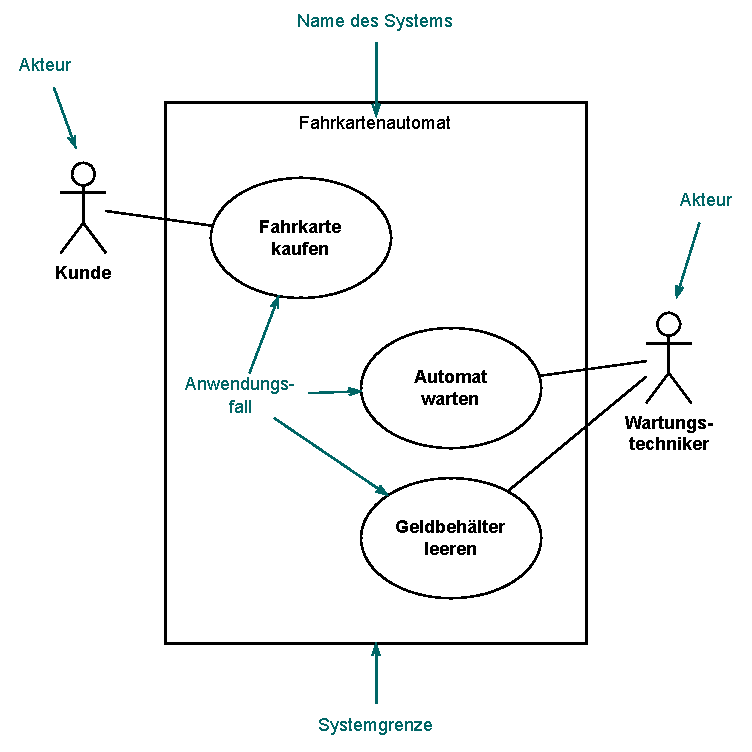
\includegraphics[scale=1.0]{Bilder/Kapitel-6/Fahrkartenautomat.pdf}	
	\caption[Ein UML-Anwendungsfalldiagramm]{Ein einfaches UML-Anwendungsfalldiagramm mit zwei Akteuren und drei Anwendungsfällen}
	\label{fig:fahrkartenautomat}
\end{figure}

Ein Anwendungsfalldiagramm besteht aus mindestens einem Anwendungsfall, der mit mindestens einem Akteur verbunden ist. Abbildung~\ref{fig:fahrkartenautomat} zeigt ein Anwendungsfalldiagramm mit zwei Akteuren (Kunde, Wartungstechniker), in UML-Notation dargestellt als Strichmännchen als Zeichen für menschliche Akteure. Außerdem sind drei Anwendungsfälle abgebildet, dargestellt als Ellipsen (keine Kreise!). Die Bezeichnung eines Anwendungsfalls wird üblicherweise als Tätigkeit formuliert.

Über die Verbindungen zwischen Akteuren und Anwendungsfällen wird modelliert, welche Akteure welche Anwendungsfälle ausführen. In der Abbildung ist der Akteur \sttpUMLText{Kunde} nur mit dem Anwendungsfall \sttpUMLText{Fahrkarte kaufen} verbunden, er kann also die beiden anderen Anwendungsfälle \sttpUMLText{Automat warten} und \sttpUMLText{Geldbehälter leeren} nicht ausführen. Dies soll nur der Akteur \sttpUMLText{Wartungstechniker} können, daher bestehen Verbindungen vom Akteur Wartungstechniker zu diesen zwei Anwendungsfällen.

Ein \marginline{Akteur} Akteur in einem Anwendungsfalldiagramm modelliert eine Rolle, die konkrete Nutzer bei der Benutzung des Systems annehmen können. Akteure bilden also keine Nutzer ab, sondern nur eingenommene Rollen bei der Systemnutzung. So könnte zum Beispiel ein realer Nutzer des Systems in der Rolle \sttpUMLText{Kunde} eine Fahrkarte kaufen, \textbf{dieselbe} Person in der Rolle \sttpUMLText{Wartungstechniker} aber auch den Automaten warten oder den Geldbehälter leeren.

Jeder Anwendungsfall in einem Anwendungsfalldiagramm, der mit Akteur(en) verbunden ist, definiert eine Interaktionsschnittstelle zwischen dem System und einem oder mehreren Akteuren. Ein Anwendungsfall beschreibt eine abgeschlossene Funktionalität, die das System erbringen muss. Dabei wird aber nicht festgelegt, \textbf{wie} diese Funktionalität erbracht werden soll und auch nicht zwangsläufig (\su) aus wie vielen und welchen einzelnen Aktionen die Interaktion zwischen Akteur(en) und System besteht. Üblicherweise bildet man die Anwendungsfälle aus Sicht der Akteure so, dass jeder Anwendungsfall einen erkennbaren Nutzen für die beteiligten Akteure erbringt. Von Einzelheiten auf dem Weg zu diesem Nutzen kann auch abstrahiert werden. So wird zum Beispiel der Anwendungsfall \sttpUMLText{Fahrkarte kaufen} vermutlich aus mehreren Interaktionen zwischen Akteur \sttpUMLText{Kunde} und dem System bestehen (\mbox{Züge} aussuchen, Tarif auswählen, Geld einzahlen etc.). Diese Menge an Aktionen wird hier in Abbildung~\ref{fig:fahrkartenautomat} in dem Anwendungsfall \sttpUMLText{Fahrkarte kaufen} gebündelt, der dem Akteur \sttpUMLText{Kunde} einen erkennbaren Nutzen, nämlich die gekaufte Fahrkarte, erbringt.

\pagebreak %%% für Druck

Da Anwendungsfälle Interaktionsschnittstellen der (späteren) Nutzer mit dem System sind, werden im Rahmen der Anforderungsermittlung in einem Anwendungsfalldiagramm nur solche Tätigkeiten der Nutzer berücksichtigt, die relevant für das System sind. Beispiel aus dem Zookontext: In der Realwelt füttert ein Tierpfleger Tiere. Ein Anwendungsfall \sttpUMLText{Tiere füttern} würde sich aber nur dann in einem Anwendungsfalldiagramm der Anforderungsermittlung für die Zooverwaltungssoftware finden, wenn die zukünftige Software diese Tätigkeit in irgendeiner Weise unterstützen (\zb automatisierte Futterbeschaffung), planen (\zb Planung der Fütterungszeiten), dokumentieren (\zb Übersicht über ausgegebene Futtermenge) etc. soll. (Bei der Nutzung von Anwendungsfalldiagrammen im Rahmen der Domänenmodellierung kann das auch anders sein, \su)

Neben den Akteuren und den Anwendungsfällen ist in Abbildung~\ref{fig:fahrkartenautomat} auch eine System\-grenze
\marginline{Systemgrenze} 
(viereckige Umrandung mit Angabe des Systemnamens) eingezeichnet. Alle Elemente, die sich innerhalb der Systemgrenze befinden, gehören zum System. Dies sind die Anwendungsfälle, für die das System entsprechende Funktionalität bereitstellen muss. Die Akteure als diejenigen, die mit dem System interagieren, werden außerhalb der Systemgrenze eingezeichnet. Wo genau sie außerhalb der System\-grenze platziert werden, ist nicht vorgegeben. Wir haben den Akteur \sttpUMLText{Kunde} in der Abbildung links des Systems und den Akteur \sttpUMLText{Wartungstechniker} rechts angeordnet. Üblicherweise orientiert man sich daran, bei welcher Platzierung sich die übersichtlichsten Verbindungen zu den Anwendungsfällen ziehen lassen.

Das Einzeichnen der Systemgrenze ins Anwendungsfalldiagramm ist nach UML-Regeln optional. Sinnvoll ist die Angabe der Systemgrenze in einem Anwendungsfalldiagramm insbesondere in den Fällen, in denen das betrachtete System nicht nur mit verschiedenen menschlichen Akteuren, sondern auch mit anderen technischen Systemen interagiert bzw. interagieren soll.

Bei den in UML-Anwendungsfalldiagrammen betrachteten Systemen kann es sich um reine Hardwaresysteme, reine Softwaresysteme oder eine Kombination von beidem handeln. Im Rahmen des Softwareengineering wird man eher selten reine Hardwaresysteme betrachten. Das in Abbildung~\ref{fig:fahrkartenautomat} dargestellte System mit Namen \sttpUMLText{Fahrkartenautomat} beinhaltet sowohl Hardware- als auch Softwarekomponenten. Anwendungsfalldiagramme abstrahieren jedoch davon, welche Komponente des (zukünftigen) Systems welchen der dargestellten Anwendungsfälle  übernehmen bzw. unterstützen soll. Insofern unterscheidet sich die Struktur eines Anwendungsfall\-diagramms für ein kombiniertes Hard-/Softwaresystem wie den Fahrkartenautomaten nicht von einem reinen Softwaresystem wie dem Online-Fahrkartenkauf in der nächsten Abbildung.

\minisec{Beziehungen zwischen Anwendungsfällen}

Abbildung~\ref{fig:fahrkartenautomat_online} zeigt für einen Anwendungsfall \sttpUMLText{Fahrkarte kaufen} ein verfeinertes Anwendungsfalldiagramm, in dem weitere typische Elemente vorkommen.

%%% Hier gehört Abbildung "fig:fahrkartenautomat_online" eigentlich hin.

Neben dem Anwendungsfall \sttpUMLText{Fahrkarte kaufen} befinden sich in dem Diagramm einige weitere als Ellipsen dargestellte Anwendungsfälle, die alle direkt oder indirekt mit \sttpUMLText{Fahrkarte kaufen} verbunden sind. Über die Beziehungstypen \sttpUMLText{<<include>>} und \sttpUMLText{<<extend>>} lassen sich inhaltliche Abhängigkeiten zwischen verschiedenen Anwendungsfällen modellieren.

\pagebreak %%% für Druck

\begin{figure}[h!]
	\begin{addmargin*}[0cm]{-\marginparwidth}
		\begin{addmargin*}[0cm]{-\marginparsep}
			\vspace{5mm} %%% für Druck
			\centering
			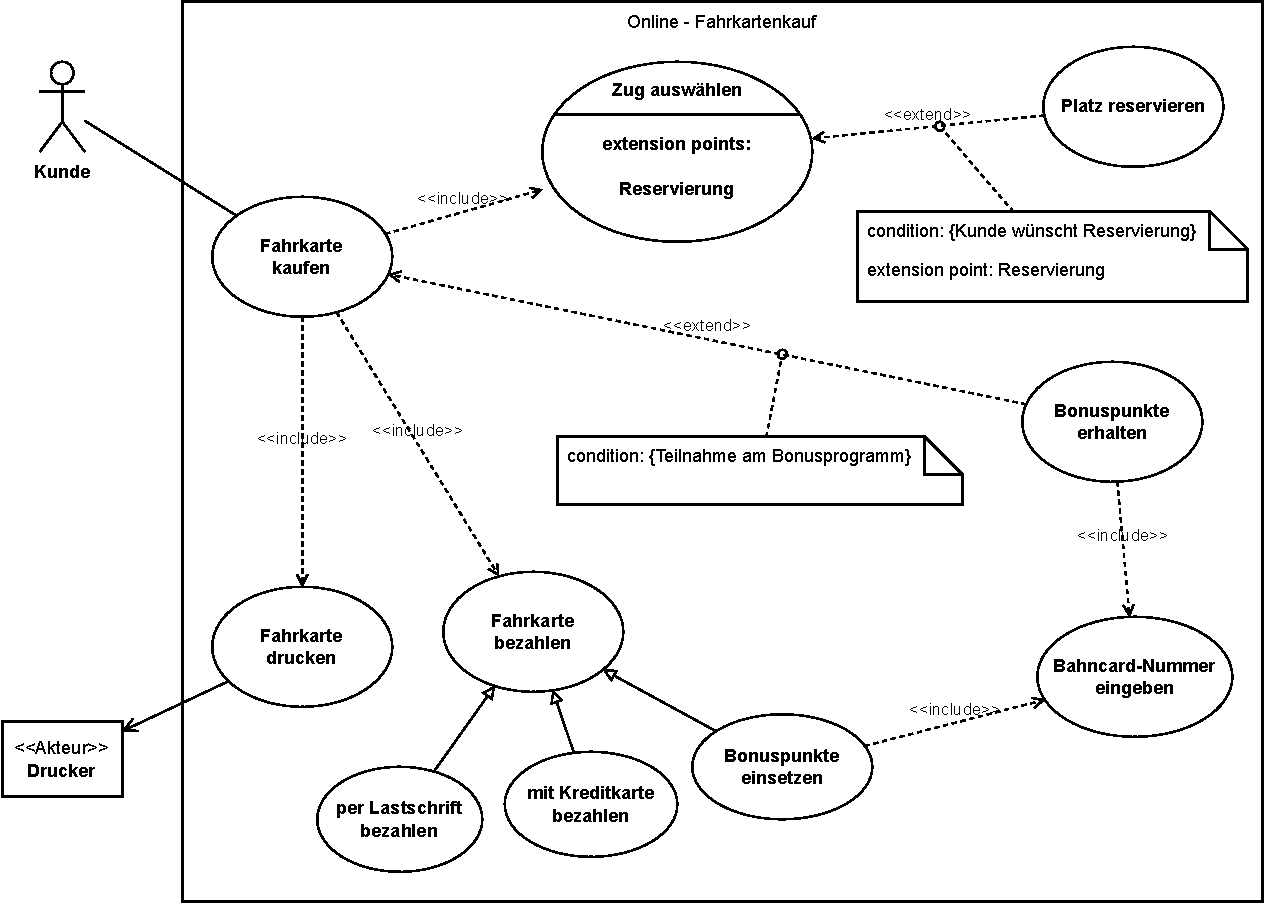
\includegraphics[scale=0.8]{Bilder/Kapitel-6/Fahrkartenautomat-online.pdf}
			\vspace{3mm} %%% für Druck
			\caption{Anwendungsfalldiagramm Online-Fahrkartenkauf}
			\label{fig:fahrkartenautomat_online}
		\end{addmargin*}
	\end{addmargin*}
\end{figure}

Alle \marginline{<<include>>} Anwendungsfälle, die über eine \sttpUMLText{<<include>>}-Beziehung mit dem Anwendungsfall \sttpUMLText{Fahrkarte kaufen} verbunden sind, gehören mit zur Funktionalität \sttpUMLText{Fahrkarte} \sttpUMLText{kaufen}. Man sagt: sie sind in die Funktionalität des Anwendungsfalls \sttpUMLText{Fahrkarte} \sttpUMLText{kaufen} \textbf{eingebunden}. In Abbildung~\ref{fig:fahrkartenautomat_online} sind also die Anwendungsfälle \sttpUMLText{Fahrkarte} \sttpUMLText{drucken}, \sttpUMLText{Fahrkarte} \sttpUMLText{bezahlen} und \sttpUMLText{Zug} \sttpUMLText{auswählen} in den Anwendungsfall
\linebreak %%% für Druck
\sttpUMLText{Fahrkarte} \sttpUMLText{kaufen} eingebunden. Die Anforderung an das zu erstellende Software\-produkt ist somit, dass jedes Mal, wenn eine Fahrkarte gekauft wird, auch alle Aktionen, die in den drei eingebundenen Anwendungsfällen spezifiziert sind, stattfinden müssen. Beachten Sie die (unter Umständen) etwas irritierende Mehrfach-Verwendung des Begriffs "`Anwendungsfall"' in Anwendungsfalldiagrammen: Jede \mbox{Ellipse} in einem Anwendungsfalldiagramm ist ein Anwendungsfall. Es wird begrifflich nicht unterschieden, ob es sich um einen eingebundenen Anwendungsfall oder um einen direkt mit dem Akteur verbundenen "`Haupt"'-Anwendungsfall handelt.

Über die Verwendung von \sttpUMLText{<<include>>} kann ein stark abstrahierter Anwendungsfall wie \sttpUMLText{Fahrkarte kaufen} in seine Teilinteraktionen zwischen Akteur und System verfeinert werden. Gleichzeitig können auf diese Weise Anwendungsfälle beschrieben werden, die identische Teilfunktionalitäten erfordern. Letztere werden dafür als eigenständiger Anwendungsfall modelliert, der in andere Anwendungsfälle eingebunden werden kann. Zum Beispiel binden die beiden Anwendungsfälle \sttpUMLText{Bonuspunkte} \sttpUMLText{erhalten} und \sttpUMLText{Bonuspunkte} \sttpUMLText{einsetzen} in Abbildung~\ref{fig:fahrkartenautomat_online} beide den Anwendungsfall \sttpUMLText{Bahncard-Nummer eingeben} ein. Genauso könnte auch ein von \sttpUMLText{Fahrkarte kaufen} völlig unabhängiger Anwendungsfall, wie zum Beispiel das Verlängern einer Bahncard, den schon im Rahmen von \sttpUMLText{Fahrkarte} \sttpUMLText{kaufen} spezifizierten Anwendungsfall \sttpUMLText{Bahncard-Nummer eingeben} einbinden. Auf diese Weise können Anwendungsfälle mit Teilfunktionalitäten für denselben oder andere Akteure wiederverwendet werden.

\vspace{1mm} %%% für Druck
 
Beachten Sie: Über die Verbindungen zwischen \sttpUMLText{Fahrkarte kaufen} und allen anderen Anwendungsfällen ist auch der Akteur \sttpUMLText{Kunde} indirekt mit allen Anwendungs\-fällen verbunden. Er kann letztere allerdings nicht unabhängig von \sttpUMLText{Fahrkarte} 
\linebreak %%% für Druck
\sttpUMLText{kaufen} initiieren. So ist zum Beispiel durch die Modellierung in Abbildung~\ref{fig:fahrkartenautomat_online} nicht vorgesehen, dass der Akteur \sttpUMLText{Kunde} einen Platz im Zug reservieren kann, ohne eine Fahrkarte zu kaufen. Sollte das eine Anforderung an das zu erstellende Software\-produkt sein, so muss der Akteur \sttpUMLText{Kunde} mit dem Anwendungsfall \sttpUMLText{Platz} \sttpUMLText{reservieren} zusätzlich direkt verbunden werden.

\vspace{1mm} %%% für Druck

Eine zweite, häufig eingesetzte Beziehungsart zwischen Anwendungsfällen ist die \sttpUMLText{<<extend>>}-Beziehung.
\marginline{<<extend>>} 
Wie die \sttpUMLText{<<include>>}-Beziehung wird sie durch einen gestrichelten Pfeil dargestellt (Vorsicht: umgekehrte Pfeilrichtung!). Die \sttpUMLText{<<extend>>}-Beziehung modelliert eine bedingte Einbindung von Anwendungsfällen, man sagt auch: sie \textbf{erweitert} den einbindenden Anwendungsfall. In Abbildung~\ref{fig:fahrkartenautomat_online} wird der Anwendungs\-fall \sttpUMLText{Fahrkarte kaufen} durch den Anwendungsfall \sttpUMLText{Bonuspunkte erhalten} erweitert. Der Anwendungsfall \sttpUMLText{Zug} \sttpUMLText{auswählen} wird durch den Anwendungsfall \sttpUMLText{Platz} \sttpUMLText{reservieren} erweitert. Die \sttpUMLText{<<extend>>}-Beziehung zwischen Anwendungsfällen wird mit einer Bedingung (engl. condition) versehen. Diese Bedingung gibt an, unter welchen Voraussetzungen der Anwendungsfall eingebunden wird. Im Gegensatz zu \sttpUMLText{<<include>>} werden also über \sttpUMLText{<<extend>>} verbundene Anwendungsfälle nicht jedes Mal eingebunden. In der Abbildung wird der Anwendungsfall \sttpUMLText{Fahrkarte kaufen} genau dann durch den Anwendungsfall \sttpUMLText{Bonuspunkte erhalten} erweitert, wenn eine Teilnahme des Akteurs am Bonusprogramm vorliegt. Sofern diese Bedingung nicht zutrifft, soll die Funktionalität hinter \sttpUMLText{Bonuspunkte erhalten} nicht Teil der Funktionalität \sttpUMLText{Fahrkarte kaufen} sein. Die UML verbietet es nicht, \sttpUMLText{<<extend>>}-Verbindungen ohne Bedingung zu modellieren. In einem solchen Fall würde der erweiternde Anwendungs\-fall immer eingebunden, sich die \sttpUMLText{<<extend>>}-Beziehung also wie eine \sttpUMLText{<<include>>}-Beziehung verhalten. Eine solche Modellierung macht das Lesen eines Anwendungsfalldiagramms aber unnötig komplizierter. Daher: wenn \sttpUMLText{<<extend>>}, dann nur zusammen mit einer Bedingung!

\vspace{1mm} %%% für Druck

Man \marginline{Erweiterungs\-punkte} kann für eine \sttpUMLText{<<extend>>}-Beziehung neben der Bedingung noch sogenannte Erweiterungspunkte (engl. extension points) angeben. In Abbildung~\ref{fig:fahrkartenautomat_online} sehen Sie diese Konstruktion in der Beziehung zwischen \sttpUMLText{Zug} \sttpUMLText{auswählen} und \sttpUMLText{Platz} \sttpUMLText{reservieren}. Dafür werden im Anwendungsfall, der erweitert wird (\sttpUMLText{Zug} \sttpUMLText{auswählen}) unter einer horizontalen Linie die möglichen Erweiterungspunkte aufgeführt und gleichzeitig am Beziehungspfeil zusätzlich zur relevanten Bedingung angegeben. Diese 
\linebreak %%% für Druck
ausführlichere Modellierung der \sttpUMLText{<<extend>>}-Beziehung ist insbesondere dann sinnvoll, wenn ein Anwendungs\-fall an mehreren \sttpUMLText{<<extend>>}-Beziehungen beteiligt ist oder es zusätzlich zur grafischen Darstellung im Diagramm eine textuelle Beschreibung (s.u.) des Anwendungs\-falls und der \sttpUMLText{<<extend>>}-Beziehung geben soll.

In UML-Anwendungsfalldiagrammen kann auch die aus den Klassendiagrammen bekannte Generalisierung verwendet werden. Damit können Hierarchien zwischen 
\linebreak %%%für Druck
Anwendungsfällen modelliert werden. In Abbildung~\ref{fig:fahrkartenautomat_online} finden sich zum Anwendungsfall \sttpUMLText{Fahrkarte bezahlen} drei „Unter“-Anwendungsfälle. Man verwendet
\linebreak %%%für Druck
Generalisierungsbeziehungen in Anwendungsfalldiagrammen immer dann, wenn eine (Teil)Funktionalität des „Ober“-Anwendungsfalls bei seinen spezialisierten Anwendungsfällen verändert ist bzw. letztere zusätzliche Funktionalität beinhalten -- also analog zur Verwendung der Generalisierung in Strukturdiagrammen wie dem Klassen\-diagramm. Generalisierungsbeziehungen kann es zudem auch zwischen Akteuren in einem Anwendungsfalldiagramm geben. Zum Beispiel könnten die Akteure \sttpUMLText{Kunde} und \sttpUMLText{Wartungstechniker} aus Abbildung~\ref{fig:fahrkartenautomat} beide Spezialisierungen eines Akteurs \sttpUMLText{Person} sein. Gene\-rali\-sierungs-Kon\-struk\-tionen auf der Ebene von Akteuren machen dann Sinn, wenn es Anwendungsfälle gibt, die mehrere bzw. alle Akteure initi\-ieren können sollen, aber gleichzeitig auch Anwendungsfälle, die nur für spezifische Akteure relevant sind. Vorsicht: auch hier sollte man wie in allen Diagrammarten die Generalisierung nicht auf die Spitze treiben. (Berühmtes Beispiel zu Generalisierungssünden: Man sollte nicht Tische von Hunden ableiten, nur weil beide vier Beine haben.)

Das letzte noch nicht besprochene Element in Abbildung~\ref{fig:fahrkartenautomat_online} ist der Akteur \sttpUMLText{Drucker} unten links. Hier sehen Sie die Modellierung für einen nicht-menschlichen Akteur. Der Akteur Drucker ist mit dem Anwendungsfall \sttpUMLText{Fahrkarte drucken} verbunden. Eine solche Verbindung mit Pfeilspitze (gerichtete Verbindung) zum Akteur wird verwendet, wenn der Akteur am Anwendungsfall beteiligt ist, diesen aber nicht selber initiieren kann. Gerichtete Verbindungen sind nicht auf nicht-menschliche Akteure beschränkt.

\vspace{2mm} %%% für Druck

\minisec{Einsatzzweck und Grenzen}

Die Abbildung~\ref{fig:fahrkartenautomat} und die Abbildung~\ref{fig:fahrkartenautomat_online} zeigen unterschiedlich stark abstrahierte Modellierungen. Beide Formen können im Rahmen der Anforderungsermittlung hilfreich sein. Über ein Anwendungsfalldiagramm wie in Abbildung~\ref{fig:fahrkartenautomat} könnte man zunächst alle direkten Interaktionen zwischen Akteuren und dem zukünftigen System spezifizieren. Jeder im Diagramm aufgeführte Anwendungsfall wäre dann mit mindestens einem Akteur direkt verbunden. Es ist im Übrigen durchaus auch üblich, pro Akteur ein eigenes Diagramm anzufertigen, in dem nur die Anwendungsfälle aufgeführt sind, die von diesem Akteur ausgeführt werden sollen. Solche Anwendungsfall\-diagramme auf einem sehr hohen Abstraktionsniveau können (zukünftige) Nutzer auch gut noch ohne Hilfe des Entwicklungsteams erstellen, insbesondere dann, wenn jeder Nutzer nur die Anwendungsfälle für seine Rolle spezifizieren muss.

Für ein schon recht verfeinertes Diagramm wie in Abbildung~\ref{fig:fahrkartenautomat_online} ist es sinnvoll, wenn Stakeholder und Entwicklungsteam (bzw. einzelne Mitglieder des Entwicklungsteams) dieses gemeinsam erstellen, um Missverständnissen von Beginn an vorzubeugen. Denn hier wird schon detaillierter festgelegt, aus welchen Teil\-inter\-aktionen eine Interaktion zwischen Akteur und System bestehen soll. Aspekte, die hier vergessen oder falsch dargestellt werden, erfordern nachher vermutlich komplexere Änderungen an diesem und unter Umständen auch weiteren Diagrammen. Gleichzeitig werden solche detaillierteren Anwendungsfalldiagramme auch eingesetzt, um gemeinsame Teil\-inter\-aktionen verschiedener Anwendungsfälle zu finden. Insbesondere wenn es sich dabei um Anwendungsfälle unterschiedlicher Akteure handelt, sollte möglichst frühzeitig sichergestellt sein, dass alle Beteiligten unter der spezifizierten Teilinteraktion wirklich das identische Verhalten vom System erwarten. 

Die Verfeinerung eines Anwendungsfalls in Teilinteraktionen ist nicht auf Anwendungsfälle beschränkt, die direkt mit Akteuren verbunden sind. Jeder Anwendungsfall in Abbildung~\ref{fig:fahrkartenautomat_online} könnte noch weiter differenziert werden. So lassen sich über Anwendungsfalldiagramme schon sehr detailliert inhaltliche Abhängigkeiten zwischen (Teil)Interaktionen erfassen. Beim praktischen Einsatz sollte man allerdings zwei Punkte beachten. Zum einen sind Anwendungsfalldiagramme nicht dazu gedacht, Reihenfolgen der Interaktionen oder zeitliche Abfolgen festzulegen. Die sicher\-lich gewünschte Reihenfolge „erst Zug auswählen, dann Fahrkarte bezahlen, dann Fahrkarte drucken“ würde man nicht über ein Anwendungsfalldiagramm ausdrücken, sondern über andere Arten von Verhaltensdiagrammen. Zum anderen sollte man den Fokus auf die Akteure nicht verlieren. Das bedeutet, jede Ellipse im Anwendungsfall\-diagramm sollte eine echte (Teil)Interaktion zwischen System und Akteur sein. Tätig\-keiten, die das System „im Hintergrund“ ausführen muss, wie zum Beispiel die Gültigkeit der Bahncard zu prüfen oder die Platzreservierung zu speichern, gehören nicht in ein Anwendungsfalldiagramm.

\vspace{1mm} %%% für Druck

\minisec{Anwendungsfalldiagramme im Rahmen der Domänenmodellierung}

Auch für die Domänenmodellierung kann man Anwendungsfalldiagramme einsetzen, zum Beispiel wie in Abbildung~\ref{fig:anwendungsfall_tiere_fuettern}, um ein besseres Verständnis von Tätigkeiten von Akteuren in der Domäne zu bekommen. Dargestellt sind hier für die Tierpfleger der Nagetiere (links) und die Tierpfleger der Löwen (rechts) die Tätigkeiten, die diese rund um die Fütterung ihrer Tiere ausführen. Das „System“, mit dem die Akteure interagieren, ist die Domäne. Die Einzeichnung von Systemgrenzen würde hier eher verwirren, da die Akteure genau wie die Anwendungsfälle Teil der Domäne sind.

%%% Hier gehört die Abbildung "fig:anwendungsfall_tiere_fuettern" eigentlich hin.

Der Einsatz von Anwendungsfalldiagrammen zur Modellierung der Domäne ist nur dann sinnvoll, wenn es einen Bezug zum zu erstellenden Softwareprodukt gibt. Hier könnte der Modellierungszweck gewesen sein, die Stellen im aktuell manuell ablaufenden Fütterungsprozess zu identifizieren, die sich für eine softwareunterstützte Automatisierung eignen würden. Die Anwendungsfälle \sttpUMLText{Futter bestellen} und \sttpUMLText{Fütterung dokumentieren} wären denkbare Kandidaten. Die Modellierung über Anwendungsfälle reicht für diese Erkenntnis auch aus und kann von den Tier\-pflegern selbst erstellt werden. Eine detaillierte und schwieriger zu erstellende Darstellung der genauen Geschäftsprozesse der Domäne (z.B. über Aktivitätsdiagramme) könnte sich für diese Anwendungsfälle dann anschließen.

\vspace{1mm} %%% für Druck

\minisec{Anwendungsfälle textuell beschreiben}

Man kann Anwendungsfälle auch textuell beschreiben. Üblicherweise findet das nicht alternativ, sondern ergänzend zu Anwendungsfalldiagrammen statt. Ziel der textuellen Ergänzung ist immer, zusätzliche Informationen festzuhalten (zu Spezifikations- oder Dokumentationszwecken), die sich nicht aus dem Diagramm allein ergeben. 

\begin{figure}[h!]
	\begin{addmargin*}[0cm]{-\marginparwidth}
		\begin{addmargin*}[0cm]{-\marginparsep}
			\vspace{5mm} %%% für Druck
			\centering
			\begin{minipage}[c]{7.5cm} 
				\centering
				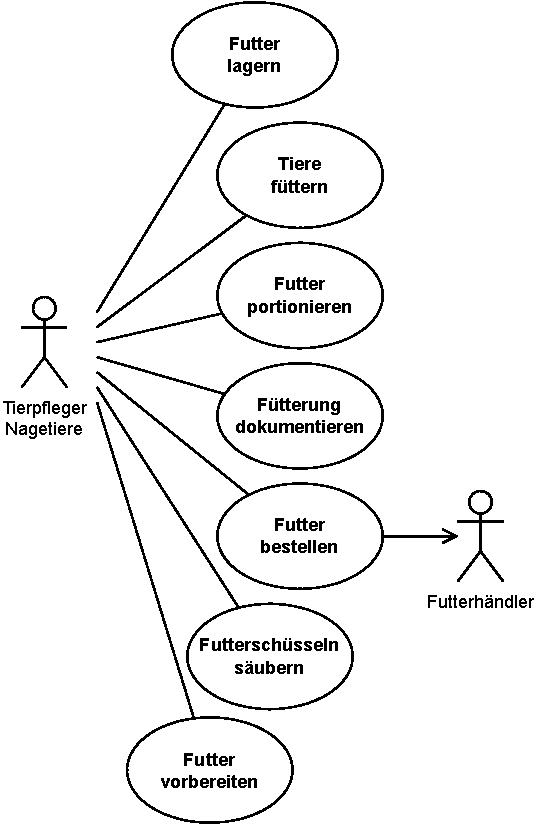
\includegraphics[scale=0.8]{Bilder/Kapitel-6/anwendungsfall_tiere_fuettern_nagetiere.pdf}
			\end{minipage}
			\begin{minipage}[c]{0.1cm} 
				\centering
				{\color{FernUni-MI-green}\rule{1pt}{90mm}} % senkrechte farbige Linie
			\end{minipage}
			\begin{minipage}[c]{9cm}
				\centering
				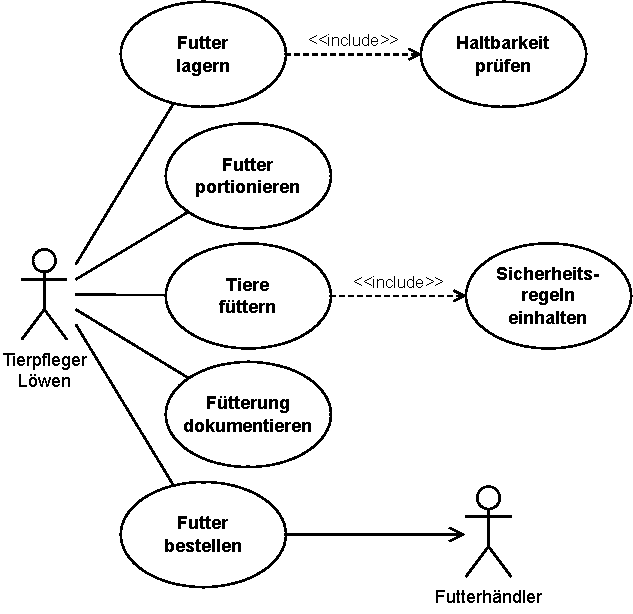
\includegraphics[scale=0.8]{Bilder/Kapitel-6/anwendungsfall_tiere_fuettern_loewen.pdf}
			\end{minipage}
			\vspace{\baselineskip} %%% für Druck
			\caption{Domänenmodellierung über Anwendungsfälle}
			\label{fig:anwendungsfall_tiere_fuettern}
		\end{addmargin*}
	\end{addmargin*}
\end{figure}

\vspace{1cm} %%% für Druck

Typische textuelle Ergänzungen sind die Angabe von Vor- und Nachbedingungen zu Anwendungsfällen oder einen Anwendungsfall auslösende Ereignisse. Zum Beispiel: Wann bzw. unter welchen Voraussetzungen wird der Anwendungsfall ausgeführt? Möglicherweise soll in Abbildung~\ref{fig:fahrkartenautomat_online} der Anwendungsfall \sttpUMLText{Fahrkarte kaufen} nur initiiert werden können, wenn der Akteur sich vorher im Buchungssystem registriert hat. 

Ein weiterer Einsatzzweck von textuellen Ergänzungen sind Erläuterungen zu im Diagramm vorkommenden Begriffen oder Konzepten. Beispiel Abbildung~\ref{fig:fahrkartenautomat_online}: Was sind Bonuspunkte? Und kann man die Bonuspunkte, die man beim Fahrkartenkauf erhalten würde direkt zum Kauf dieser Fahrkarte schon einsetzen? Ob man solche \mbox{Informationen} besser als textuelle Ergänzung zu einem Anwendungsfall-
\linebreak %%% für Druck
diagramm oder an anderer Stelle (z.B. textuell in einem Glossar oder in stärker ablauf\-orientierten anderen grafischen Diagrammen) festhält, ist sehr projektspezifisch -- in manchen agilen Vorgehensmodellen würde man sie gar nicht schriftlich festhalten, sondern nur mündlich kommunizieren.

Textuelle Ergänzungen werden häufig auch dafür verwendet, die Erweiterungen zum Standardablauf eines „Haupt“-Anwendungsfalls (alle Anwendungsfälle, die mit \mbox{<<extend>>} angebunden sind) detaillierter zu beschreiben. Auch hier gilt, dass als \mbox{Alternative} zur textuellen Ergänzung eines Anwendungsfalldiagramms auch der zusätzliche Einsatz anderer Verhaltensdiagramme (wie z.B. Aktivitätsdiagramme) 
\linebreak %%% für Druck
möglich ist.

Wenn man textuelle Ergänzungen zu Anwendungsfalldiagrammen sehr strukturiert und ausführlich aufschreiben möchte, findet man in der Literatur dafür zahlreiche Schablonen. Abbildung~\ref{fig:use_case_schablone} zeigt eine solche Schablone. Etwas anders strukturierte Schablonen finden Sie bei \cite[S. 172 und S. 193]{rup14} und \cite[98 \psq]{ber18}, bei letzterem auch Verweise auf weitere Literatur.

\vspace{\baselineskip} %%% für Druck

\begin{figure}[h!]
	\begin{addmargin*}[0cm]{-\marginparwidth}
	\begin{addmargin*}[0cm]{-\marginparsep}
		\centering
		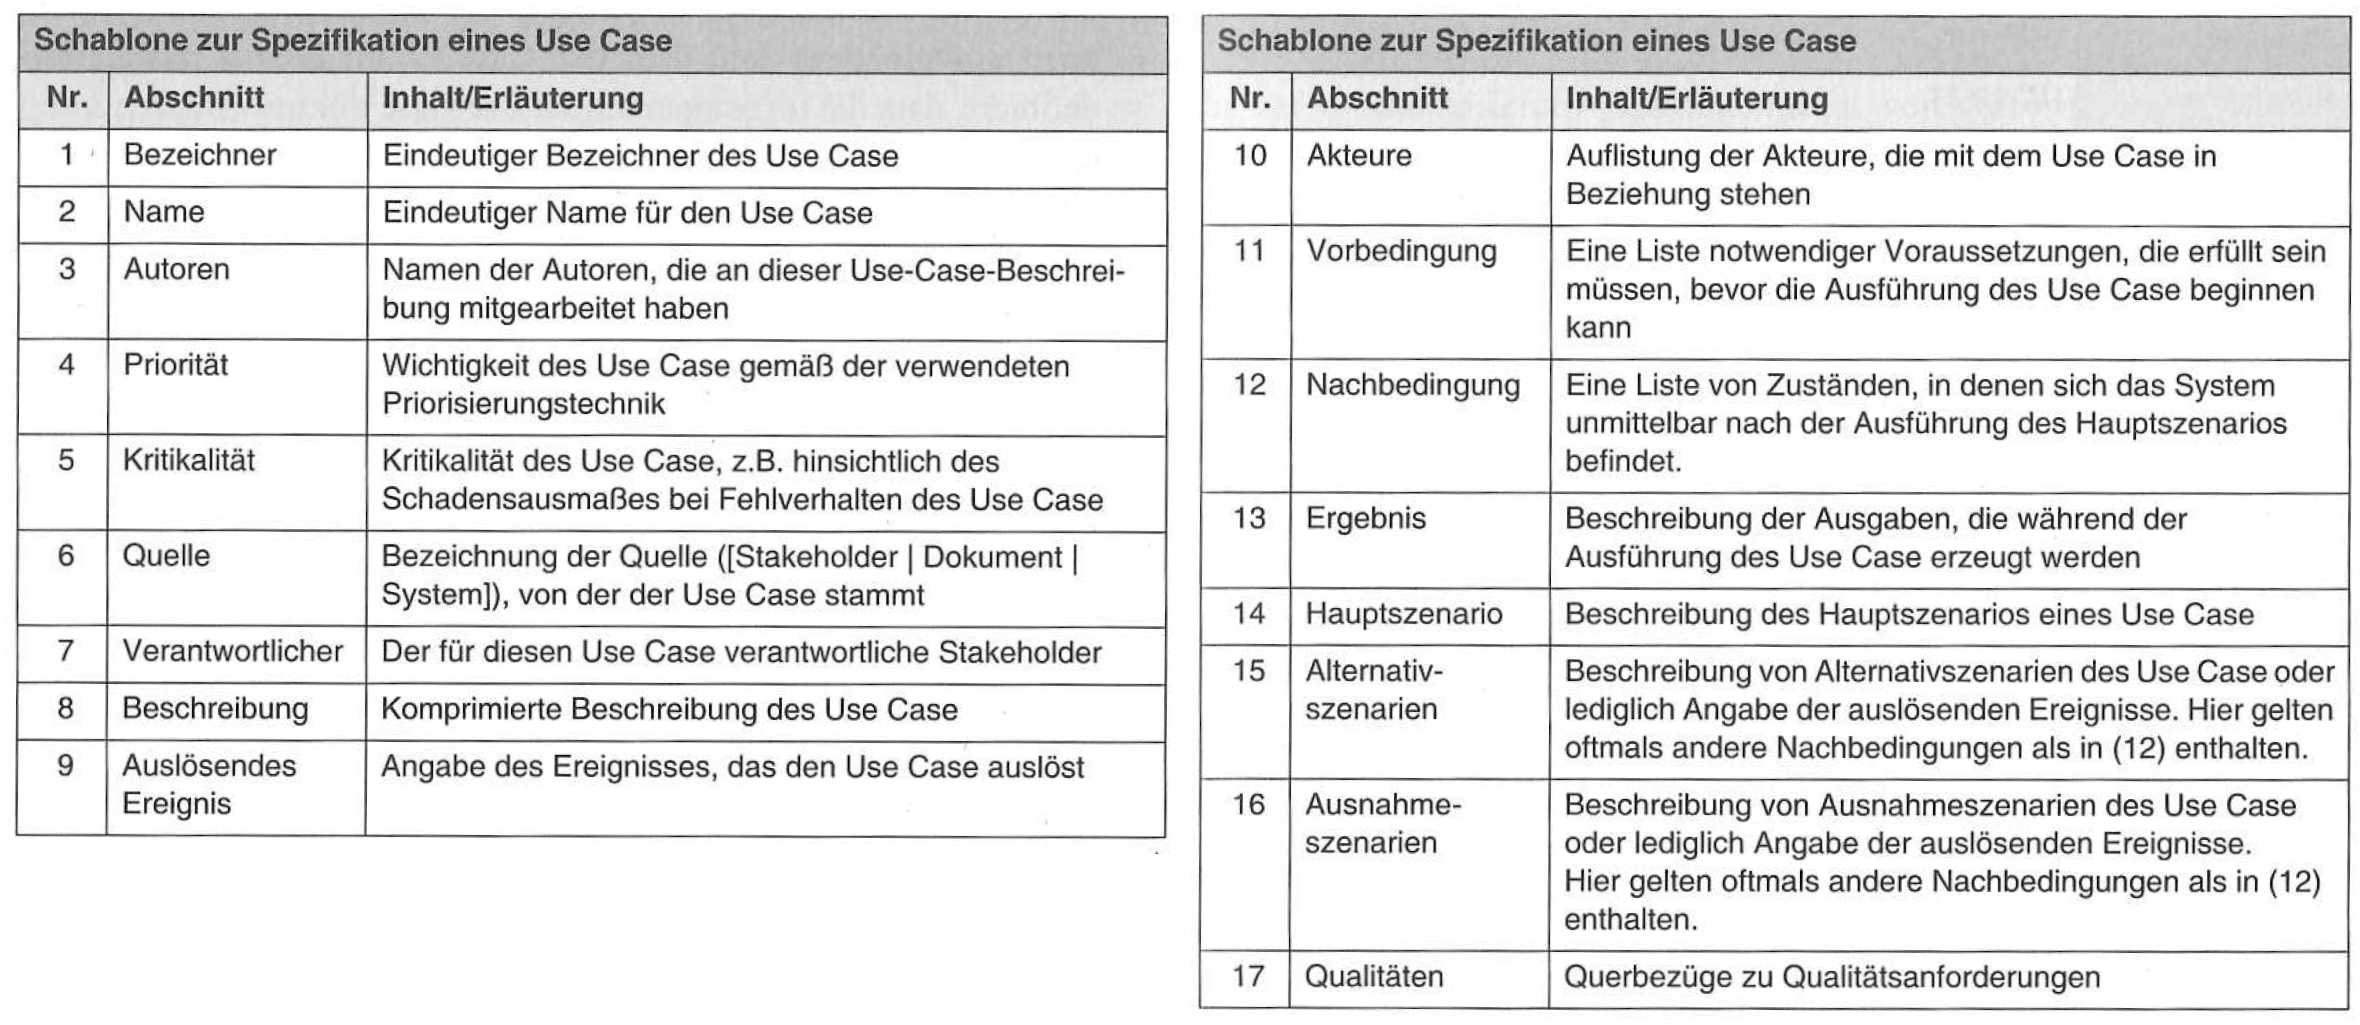
\includegraphics[scale=0.88]{Bilder/Kapitel-6/use_case_schablone.png}
		\caption[Use Case Schablone]{Use Case Schablone \cite[72 \psq]{poh15}}
		\label{fig:use_case_schablone}
	\end{addmargin*}
	\end{addmargin*}
\end{figure}

\vspace{\baselineskip} %%% für Druck

\minisec{Anwendungsfälle und User Stories}
Wir hatten in Abschnitt~\ref{sec:Kap-6.2.3} die aus dem agilen Umfeld stammenden User \mbox{Stories} angesprochen, über die sich ebenfalls die gewünschte Systemnutzung der Nutzer modellieren lässt. Anwendungsfalldiagramme und User Stories lassen sich durchaus kombinieren, zum Beispiel indem User Stories als textuelle Ergänzung zu den „Haupt“-Anwendungsfällen eines Anwendungsfalldiagramms fungieren. Wenn man den Schwerpunkt umgekehrt eher auf die User Stories setzen möchte, kann man das Anwendungsfalldiagramm als grafische Ergänzung verwenden, zum Beispiel für eine Übersicht zusammengehöriger User Stories.

\vspace{\baselineskip} %%% für Druck